%%%%%%%%%%%%%%%%%%%%%%%%%%%%%%%%%%%%%%%%%
% Short Sectioned Assignment
% LaTeX Template
% Version 1.0 (5/5/12)
%
% This template has been downloaded from:
% http://www.LaTeXTemplates.com
%
% Original author:
% Frits Wenneker (http://www.howtotex.com)
%
% License:
% CC BY-NC-SA 3.0 (http://creativecommons.org/licenses/by-nc-sa/3.0/)
%
%%%%%%%%%%%%%%%%%%%%%%%%%%%%%%%%%%%%%%%%%

%----------------------------------------------------------------------------------------
%	PACKAGES AND OTHER DOCUMENT CONFIGURATIONS
%----------------------------------------------------------------------------------------

\documentclass[paper=a4, fontsize=11pt]{scrartcl} % A4 paper and 11pt font size

\usepackage[T1]{fontenc} % Use 8-bit encoding that has 256 glyphs
%\usepackage{fourier} % Use the Adobe Utopia font for the document - comment this line to return to the LaTeX default
\usepackage[english]{babel} % English language/hyphenation
\usepackage{amsmath,amsfonts,amsthm} % Math packages
\usepackage{mathtools} %More math! (For dscases)
\usepackage{hyperref} %HTML package
\usepackage{pgfplots} %Makes plots in LaTeX
\usepackage{tikz} %Also tikz?
\usepackage{bbm} %Blackboard bold 1
\usepgfplotslibrary{fillbetween}%Let's me fill between named plots
\usepackage{graphicx} %import pics
\graphicspath{ {Python_figs/} }
\DeclareGraphicsExtensions{.pdf,.png,.jpg}
\usepackage{sectsty} % Allows customizing section commands
\allsectionsfont{ \normalfont\scshape} % Make all sections the default font and small caps


\renewcommand{\thesubsection}{\alph{subsection}} %Make subsections start with letters

\usepackage{fancyhdr} % Custom headers and footers
\pagestyle{fancyplain} % Makes all pages in the document conform to the custom headers and footers
\fancyhead{} % No page header - if you want one, create it in the same way as the footers below
\fancyfoot[L]{} % Empty left footer
\fancyfoot[C]{} % Empty center footer
\fancyfoot[R]{\thepage} % Page numbering for right footer
\renewcommand{\headrulewidth}{0pt} % Remove header underlines
\renewcommand{\footrulewidth}{0pt} % Remove footer underlines
\setlength{\headheight}{13.6pt} % Customize the height of the header

\numberwithin{equation}{section} % Number equations within sections (i.e. 1.1, 1.2, 2.1, 2.2 instead of 1, 2, 3, 4)
\numberwithin{figure}{section} % Number figures within sections (i.e. 1.1, 1.2, 2.1, 2.2 instead of 1, 2, 3, 4)
\numberwithin{table}{section} % Number tables within sections (i.e. 1.1, 1.2, 2.1, 2.2 instead of 1, 2, 3, 4)

\setlength\parindent{0pt} % Removes all indentation from paragraphs - comment this line for an assignment with lots of text

%----------------------------------------------------------------------------------------
%	TITLE SECTION
%----------------------------------------------------------------------------------------

\newcommand{\horrule}[1]{\rule{\linewidth}{#1}} % Create horizontal rule command with 1 argument of height

\title{	Assignment 9}

\author{Benjamin Jakubowski} % Your name

\date{\normalsize\today} % Today's date or a custom date

\begin{document}

\maketitle % Print the title

%----------------------------------------------------------------------------------------
%	PROBLEM 1
%----------------------------------------------------------------------------------------

\section{True or False}

\subsection{Projection of $x$}

The statement "\emph{the projection of a vector on a subspace $S$ is equal to}
\[\mathcal{P}_{S} x = \sum_{i=1}^{n} \langle x, b_i \rangle b_i \]
\emph{for any basis $b_1, ...., b_n$ of $S$}" is false. \\
\textbf{Counterexample}: \\
Let
\begin{itemize}
\item $V = R^2$
\item $S = \textrm{span}\left\{ s \right\} = \textrm{span}\left\{\left[ \begin{matrix} 2 \\ 0 \end{matrix}\right]\right\}$.
\item $ x = \left[ \begin{matrix} 1 \\ 1 \end{matrix}\right]$.
\end{itemize}

Then $\langle x, s \rangle x = (1\cdot 2 + 1\cdot 0 ) \cdot \left[ \begin{matrix} 2 \\ 0 \end{matrix}\right] = \left[ \begin{matrix} 4 \\ 0 \end{matrix}\right]$.

But then
\[x - \langle x, s \rangle s = \left[ \begin{matrix} 1 \\ 1 \end{matrix}\right] - \left[ \begin{matrix} 4 \\ 0 \end{matrix}\right] = \left[ \begin{matrix} -3 \\ 1 \end{matrix}\right] \notin S^{\bot}\]

We can understand this visually:\\
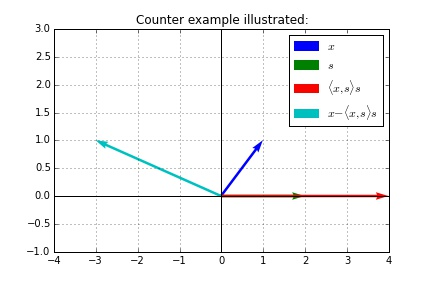
\includegraphics[scale = 1]{q1_a.jpg}\\
Since $s$ is not normal, $\langle x , s \rangle s$ is \textbf{not} the projection of $x$ on $s$. Instead, we'd need to define
\[ \mathcal{P}_S x := \langle x, s \rangle \frac{s}{||s||_2}\]

\subsection{Orthogonal complements}

The statement "\emph{the orthogonal complement of the orthogonal complement of a subspace $S$ is $S$}" is true.

\textbf{Proof}:\\
First, take $y \in S$. By definition, $\langle y, x \rangle = 0$ for all $x \in S^\bot$. Thus (again applying the definition of orthogonal complement) $y \in \left(S^\bot\right)^\bot$, so $S \subseteq \left(S^\bot\right)^\bot$.

Finally, take $v \in \left(S^\bot\right)^\bot$. Since $v \in V$ (and $S$ is a subspace), we can write
\[ v = \mathcal{P}_{S^\bot} v + \mathcal{P}_{S} v \]
Since $v \in \left(S^\bot\right)^\bot$, $\mathcal{P}_{S^\bot} v = 0 $ so $v = \mathcal{P}_{S} v $ and $v \in S$. Thus $\left(S^\bot\right)^\bot \subseteq S$, so $\left(S^\bot\right)^\bot = S$.

\subsection{Power method convergence}

The statement "\emph{... the power method converges to a vector in the span of $\{v_1\}$ no matter how you initialize it"} is false.

\textbf{Counterexample}:\\

Recall $A \in \mathbb{R}^n$ has $n$ eigenvalues $\lambda_1 > \lambda_2 > ... > \lambda_n$ corresponding to $n$ linearly independent eigenvectors $v_1, v_2, ..., v_n$.

Now let $x = \sum_{i = 1}^n \alpha_i Q_{:i}$ be the initializing vector for the power method (where $Q_{:i}$ is the $i^{th}$ column in $A = Q \Lambda Q^{-1}$ or equivalently the $i^{th}$ eigenvector).

Then (by (66) on page 10 of the notes),
\[A^k x = \sum_{i = 1}^n \alpha_i \lambda_i^k Q_{:i}\]
Now, if $\alpha_1 = 0$, then
\[A^k x = \sum_{i = 1}^n \alpha_i \lambda_i^k Q_{:i} = \sum_{i = 2}^n \alpha_i \lambda_i^k Q_{:i}\]

Then, as $k \to \infty$ the term $\alpha_2 \lambda_2^k Q_{:2}$ will dominate. Thus, if you happen to (completely improbably) initialize the power method with $x \in \textrm{span}\{v_1\}^\bot$ it will not converge to a vector in $\textrm{span}\{v_1\}$ but instead to a vector in $\textrm{span}\{v_2\}$.

%----------------------------------------------------------------------------------------
%	PROBLEM 2
%----------------------------------------------------------------------------------------

\section{Heartbeat}

\subsection{Finding a basis for span of $Y_1$ and $Y_2$}

First, recall we are given:
\begin{itemize}
\item $Y_1 = B + M$
\item $Y_2 = M + N$
\item $E(M) = E(B) = E(N) = 0 \implies E(Y_1) = E(Y_2) = 0$
\item $Var(B) = Var(N) = \sigma^2, Var(M) = 3\sigma^s$
\item $Cov(B,N) = Cov(N,M) = Cov(B,M) = 0$
\end{itemize}

We want to find an orthonormal basis for $\textrm{span}\{Y_1, Y_2\}$.

First note:
\begin{align*}
Var(Y_1) &= Var(B+M) = Var(B) + Var(M) \qquad{} \textrm{(since uncorrelated)} \\
   &= \sigma^2 + 3\sigma^2 = 4\sigma^2
\end{align*}
Similarly,
\begin{align*}
Var(Y_2) &= Var(M + N) = Var(M) + Var(N) \qquad{} \textrm{(since uncorrelated)} \\
   &= 3\sigma^2 + 1\sigma^2 = 4\sigma^2
\end{align*}
Next,
\begin{align*}
Cov(Y_1, Y_2) &= E(Y_1Y_2) - E(Y_1)E(Y_2) \\ 
   &= E(Y_1 Y_2) \\
   &= E\left((B + M)(M + N)\right) \\
   &= E\left(B M + M^2 + B N + M N\right) \\
   &= E(B M) + E(M^2) + E(B N) + E(M N) \\
   &= 0 + E(M^2) + 0 + 0 \\
   &= 3\sigma^2
\end{align*}

Now let's use Gram-Schmidt to find a basis for $\textrm{span}\{Y_1, Y_2\}$. First we'll find a basis- then we'll normalize the basis vectors to produce an orthonormal basis.

Let $U_1 = Y_1$.

Then let
\begin{align*}
U_2 &= Y_2 - \frac{\langle Y_2, U_1 \rangle}{\langle U_1, U_1 \rangle}U_1 \\
   &=Y_2 - \frac{\langle Y_2, Y_1 \rangle}{\langle Y_1, Y_1 \rangle}Y_1 \\
   &= Y_2 - \frac{ E(Y_1Y_2)}{E(Y_1^2)}Y_1 \\
   &= Y_2 - \frac{ Cov(Y_1,Y_2)}{Var(Y_1)}Y_1 \\
   &= Y_2 - \frac{ 3\sigma^2}{4 \sigma^2}Y_1 \\
   &= Y_2 - \frac{ 3}{4}Y_1
\end{align*}

So our (non-orthonormal) basis for $\textrm{span}\{Y_1, Y_2\}$ is $\{Y_1, Y_2 - \frac{ 3}{4}Y_1\}$.

Now we normalize these basis vectors to produce an orthonormal basis:
\begin{align*}
V_1 &= \frac{U_1}{\sqrt{\langle U_1, U_1 \rangle}} =  \frac{Y_1}{\sqrt{Var(Y_1)}} = \frac{Y_1}{2\sigma} \\
V_2 &= \frac{U_2}{\sqrt{\langle U_2, U_2 \rangle}} =  \frac{Y_2 - \frac{ 3}{4}Y_1}{\sqrt{Var(Y_2 - \frac{ 3}{4}Y_1)}}
\end{align*}

Thus, to proceed, we first need to find $Var(Y_2 - \frac{ 3}{4}Y_1)$.
\begin{align*}
Var\left(Y_2 - \frac{ 3}{4}Y_1\right) &= Var(Y_2) + \left(\frac{-3}{4}\right)^2 Var(Y_1) + 2 \left(\frac{-3}{4}\right) Cov(Y_1,Y_2)\\
   &= 4 \sigma^2 + \frac{9}{4}\sigma^2 - \frac{3}{2} \cdot 3 \sigma^2 \\
   &= \left(4 + \frac{9}{4} - \frac{9}{2}\right) \sigma^2 \\
   &= 7/4 \sigma^2
\end{align*}
Thus, 
\begin{align*}
V_1 &=  \frac{Y_1}{2\sigma} \\
V_2 &= \frac{Y_2 - \frac{ 3}{4}Y_1}{\sqrt{Var(Y_2 - \frac{ 3}{4}Y_1)}} = \frac{Y_2 - \frac{ 3}{4}Y_1}{\sqrt{7/4 \sigma^2}} \\
   &= \frac{2}{\sqrt{7}\sigma} Y_2 - \frac{3}{2\sqrt{7}\sigma}Y_1
\end{align*}

So, our final orthonormal basis for $\textrm{span}\{Y_1, Y_2\}$ is $\left\{\frac{1}{2\sigma}Y_1, \frac{2}{\sqrt{7}\sigma} Y_2 - \frac{3}{2\sqrt{7}\sigma}Y_1\right\}$.

\subsection{Best linear estimator}

We want to find the best linear estimator $\hat{B}_{LMMSE}$ given $Y_1$ and $Y_2$. This is
\[ \arg \min_{\hat{B}} E\left( (\hat{B} - B)^2 \right) \]
subject to $ \hat{B} = aY_1 + BY_2 + c$ for $a, b, c \in \mathbb{R}$.\\

\textbf{\emph{Note: I solved this problem rather circuitously at first. Then I realized I could solve it much more simply by projecting on the basis found in part (a). Instead of just deleting my first attempt (which is also correct), I've decided to present both}}

\subsubsection{Find $\hat{B}_{LMMSE}$ through explicit minimization}

The cost function is
\begin{align*}
h(a,b,c) &= E\left( (\hat{B} - B)^2 \right) \\
   &= E\left( (aY_1 + bY_2 + c - B)^2 \right) \\
   &= E\left( (a(B+M) + b(M+N) + c - B)^2 \right) \\
   &= E\left( ((a-1) B + (a+b) M + bN + c)^2 \right) \\
   &= E\left( (a-1)^2 B^2 + (a+b)^2 M^2 + b^2 N^2 + c^2 \right) \qquad{^*(\emph{see below for justification})}\\
   &= (a-1)^2 E(B^2) + (a+b)^2 E(M^2) + b^2 E(N^2) + c^2
\end{align*}
  * Note in expanding this quadratic polynomial we can drop all cross terms (of form $kXY$ for $k \in \mathbb{R} \textrm{ and } X, Y \in \{B, M, N\}, X \ne Y$) since these random variables are all uncorrelated. We can also drop all terms of the form $kX$ since all the random variables are zero mean.
  
Note this expression is clearly minimized when $c = 0$. Thus the cost function becomes
\begin{align*}
h(a,b) &= (a-1)^2 E(B^2) + (a+b)^2 E(M^2) + b^2 E(N^2) \\
   &= (a-1)^2 \sigma^2 + (a+b)^2 3 \sigma^2 + b^2 \sigma^2 \\
   &= \left[ (a-1)^2 + 3(a+b)^2 + b^2\right] \sigma^2
\end{align*}
Now we find the minimum of this function by setting the partials to zero and evaluating:
\begin{align*}
\frac{\delta h}{\delta a} &= \left[ 2(a-1) + 6(a+b) \right] \sigma^2 = 0 \\
\frac{\delta h}{\delta b} &= \left[ 6(a+b) +2b \right] \sigma^2 = 0
\end{align*}
Thus 
\begin{align*}
8a + 6b - 2 &= 0 \\
\implies 4a + 3b &= 1
\end{align*}
and
\begin{align*}
6a + 8b &= 0 \\
\implies a &= -4/3 b
\end{align*}
Substituting yields
\begin{align*}
4(-4/3b) + 3b &= 1 \\
\implies -16b + 9b &= 3\\
\implies b &= -3/7
\end{align*}
so $a = 4/7$. 

Before we proceed, let's check this is in fact a minimum:
\begin{align*}
\textrm{det} \left[\begin{matrix} \frac{\delta^2 h}{\delta a^2} & \frac{\delta^2 h}{\delta a \delta b} \\ \\
   \frac{\delta^2 h}{\delta b \delta a} & \frac{\delta^2 h}{\delta b^2} \end{matrix} \right]  &= \textrm{det} \left[\begin{matrix} 8 \sigma^2 & 6 \sigma^2 \\
   6 \sigma^2 & 8 \sigma^2 \end{matrix} \right] \\
   &= 8^2 \sigma^4 - 6^2 \sigma^4 = 28 \sigma^4 > 0
\end{align*}
So it is in fact a minimum. Thus

\[\hat{B}_{LMMSE} =4/7 \cdot Y_1 - 3/7 \cdot Y_2\]

\subsubsection{Find $\hat{B}_{LMMSE}$ through projection}

Now for the better answer. By definition, $\hat{B}_{LMMSE}$ is just the projection of $B$ onto the subspace spanned by $Y_1$ and $Y_2$. Hence we can use the orthonormal basis found in part (a) to easily find $\hat{B}_{LMMSE}$:
\[
\mathcal{P}_{\textrm{span}\{Y_1,Y_2\}} B = \langle \frac{1}{2\sigma}Y_1, B \rangle \frac{1}{2\sigma}Y_1 + \langle  \frac{2}{\sqrt{7}\sigma} Y_2 - \frac{3}{2\sqrt{7}\sigma}Y_1, B \rangle \left(\frac{2}{\sqrt{7}\sigma} Y_2 - \frac{3}{2\sqrt{7}\sigma}Y_1\right) \\
 \]
 Since $Cov(M,B) = Cov(N,B) = 0$, this becomes
\begin{align*}
\mathcal{P}_{\textrm{span}\{Y_1,Y_2\}} B &= \langle \frac{1}{2\sigma}B, B \rangle \frac{1}{2\sigma}Y_1 + \langle  \frac{-3}{2\sqrt{7}\sigma} B, B \rangle \left(\frac{2}{\sqrt{7}\sigma} Y_2 - \frac{3}{2\sqrt{7}\sigma}Y_1\right) \\
   &= \frac{1}{4} Y_1 - \frac{3}{2 \sqrt{7}\sigma} \cdot \sigma^2 \left(\frac{2}{\sqrt{7}\sigma} Y_2 - \frac{3}{2\sqrt{7}\sigma}Y_1\right) \\
   &= \frac{1}{4} Y_1 - \frac{3}{7} Y_2 + \frac{9}{28} Y_1 \\
   &= \frac{4}{7} Y_1 - \frac{3}{7} Y_2
\end{align*}

This is a much more elegant solution, because it immediately lends itself to a geometric interpretation- $\hat{B}_{LMMSE}$ is the closest vector to $B$ in the subspace $\textrm{span}\{Y_1, Y_2\}$. 

%----------------------------------------------------------------------------------------
%	PROBLEM 3
%----------------------------------------------------------------------------------------

\section{Cold}

\subsection{Probability Bob has a cold today}

Let's assume the following
\begin{enumerate}
\item Bob's age in days is large.
\item This process is well modeled as a time-invariant Markov process.
\end{enumerate}
Additionally let
\begin{itemize}
\item $T = s$ if sick today, $T = w$ if well today
\item $Y = s$ if sick yesterday, $Y = w$ if well yesterday
\end{itemize}
Then, the transition matrix is
\[P = \left[
\begin{matrix}
P(T = s | Y = s) & P(T = s | Y = w) \\
P(T = w | Y = s) & P(T = w | Y = w) \\
\end{matrix} \right]
= \left[
\begin{matrix}
0.8 & 0.1 \\
0.2 & 0.9 \\
\end{matrix} \right]
\]
If Bob is indeed old, we can assume this Markov process has converged to its steady state (corresponding to $\lambda_1 = 1$). Thus,
\[ v_1 =\left[ \begin{matrix}P(T = s) \\ P(T = w) \end{matrix} \right] =  \left[ \begin{matrix} P(Y = s) \\ P(Y = w) \end{matrix} \right] \]
such that
\begin{align*}
P v_1  &=v_1 \\
(\mathbb{I}_2 - P) v_1 &= 0 \\
\left[ \begin{matrix} .2 & -.1 \\ -.2 & .1 \\ \end{matrix} \right] v_1 &= 0
\end{align*}
Now recalling $v_1 = \left[ \begin{matrix} P(T = s) \\ P(T = w) \end{matrix} \right]$, we know:
\begin{align*}
.2P(T = s) - 0.1P(T = w) &= 0 \\
\implies \qquad{} 0.2P(T = s) &= 0.1P(T = w) \\
\implies \qquad{} P(T = s) &= 1/2 P(T = w) \\
\end{align*}
Finally, since $v_1$ is a PMF, we know $P(T = s) + P(T = w) = 1$. Hence, under our assumptions, $P(T = s) = 1/3$.

\subsection{Probability Bob had a cold three days ago}

Now we know Bob has a cold today. We're interested in predicting whether he was sick three days ago. First, let
\[
D_{3} = \begin{cases}
s & \textrm{if sick three days ago}\\
w & \textrm{if well three days ago}
\end{cases}
\]
Then we know our MAP estimate for $D_{3}$ is
\[\hat{D_{3}}_{MAP} = \arg \max_{x \in \{s, w\}} P(D_{3} = x | T = s) \]

But (using Bayes rule)
\[P(D_{3} = x | T = s) = c \cdot P(D_{3} = x)P(T = s | D_{3} = x)\]
where $c$ is the inverse probability of the evidence (a constant that does not effect our MAP estimate).

Next, we find $P(T = s | D_{3} = x)$. Note we find this probability by first determining the vector $\left[\begin{matrix} P(T = s | D_{3} = x) \\ P(T = w | D_{3} = x) \end{matrix} \right]$ for $x \in \{s, w\}$.
\[
\left[\begin{matrix} P(T = s | D_{3} = x) \\ P(T = w | D_{3} = x) \end{matrix} \right] =
\begin{cases}
P^3 \left[\begin{matrix}1 \\ 0 \end{matrix}\right] & \textrm{ if } x = s\\
P^3 \left[\begin{matrix}0 \\ 1 \end{matrix}\right] & \textrm{ if } x = w\\
\end{cases}
\]
Using WolframAlpha, we find $P^3 = \left[ \begin{matrix} 0.526 & 0.219 \\ 0.438 & 0.781 \end{matrix} \right]$. Thus
\[
\left[\begin{matrix} P(T = s | D_{3} = x) \\ P(T = w | D_{3} = x) \end{matrix} \right] =
\begin{cases}
\left[\begin{matrix} 0.561 \\ 0.438 \end{matrix}\right] & \textrm{ if } x = s\\
\left[\begin{matrix} 0.219 \\ 0.781 \end{matrix}\right] & \textrm{ if } x = w\\
\end{cases}
\]
Thus
\[
P(T = s | D_{3} = x) =
\begin{cases}
0.561 & \textrm{ if } x = s \\
0.219 & \textrm{ if } x = w
\end{cases}
\]
Finally,  note (again under our steady state approximation) $P(D_{3} = s) = 1/3$ and $ P(D_{3} = w) = 2/3$. Hence,
\[
 c \cdot P(D_{3} = x)P(T = s | D_{3} = x) = 
 \begin{cases}
 c \cdot 1/3 \cdot 0.561 = 0.187 c & \textrm{ if } x = s \\
 c \cdot 2/3 \cdot 0.219 = 0.146 c & \textrm{ if } x = w \\
\end{cases}
\]
Thus, our MAP estimate for $D_{3}$ is
\[\hat{D_{3}}_{MAP} = s\]
and our probability of error is $\frac{0.146 c}{0.146 c + 0.187 c} = 43.8\%$.

%----------------------------------------------------------------------------------------
%	PROBLEM 4
%----------------------------------------------------------------------------------------

\section{PCA of Wheat data}

\subsection{Projecting the seeds data onto different principle components}

\subsubsection{Projecting onto principle components [1] and [2]}
The projection of the seeds data onto principle components [1] and [2] is shown below:
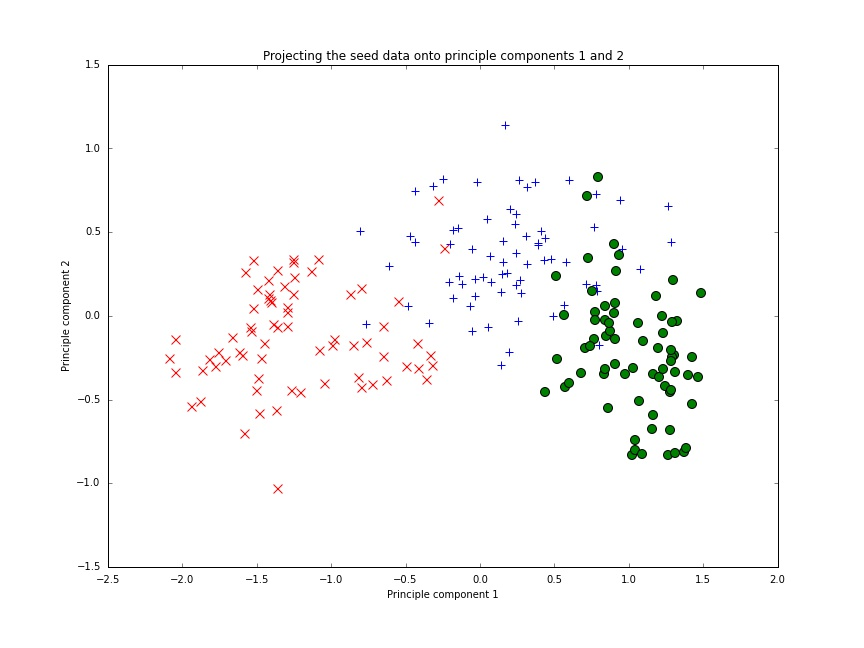
\includegraphics[scale = 0.5]{q4_ai.jpg}
As you can see, the three seed varietals are well-discriminated when projected onto the first two principle components.

\subsubsection{Projecting onto principle components [-2] and [-1]}
The projection of the seeds data onto principle components [-2] and [-1] is shown below:
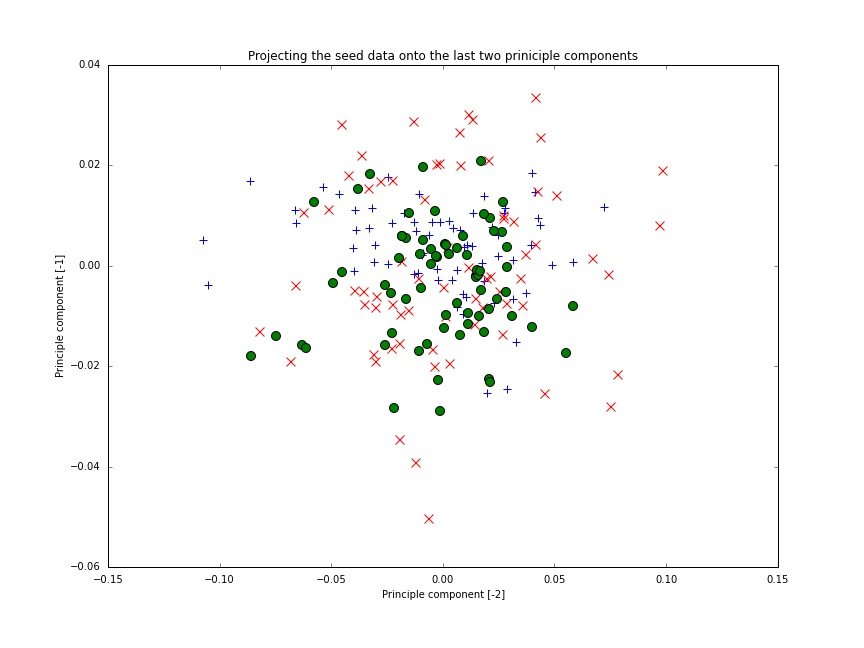
\includegraphics[scale = 0.5]{q4_aii.jpg}
As you can see, the three seed varietals are poorly discriminated when projected onto the last two principle components. This is as expected (assuming the predictors are in fact informative). The first two principle components capture the majority of the variance (energy), while the last two components capture very little (and, as such, are essentially describing noise dimensions in the predictor space). 

\subsection{Using SVD for learning}

Imagine we have a training set and a test set. To classify the seeds of the test set using dot products and the SVD, I would:
\begin{enumerate}
\item Break the training set into k folds (perhaps k=10) for cross validation.
\item Determine the singular value decomposition for the x-validation training set.
\item Iteratively project the hold-out set onto the first $i \in \{1, ..., n\}$ principal components. For each $i$, classify each observation $y$ in the hold-out x-validation set as $$\arg \min_{\textrm{Variety} \in \{\textrm{Kama, Rosa, Canadian}\}} ||y -  \bar{x}_{variety}||_2 $$ and determine the accuracy (or performance under some other evaluation metric). Note that here $\bar{x}_{variety}$ is the mean vector for each variety.
\item Pick the number $j$ of principal components that minimize the loss function (i.e. minimize 0-1 loss), averaged over the k-folds.
\item Determine the singular value decomposition for the entire dataset. Then take the first $j$ principal components, project the test set observations on these components, and use the same classification method described above to classify each observation.
\end{enumerate}
%----------------------------------------------------------------------------------------
\end{document}